\documentclass{beamer}
\mode<presentation>
\usepackage{amsmath}
\usepackage{amssymb}
%\usepackage{advdate}
\usepackage{graphicx}
\graphicspath{{./figs/}}
\usepackage{adjustbox}
\usepackage{subcaption}
\usepackage{enumitem}
\usepackage{multicol}
\usepackage{mathtools}
\usepackage{listings}
\usepackage{url}
\def\UrlBreaks{\do\/\do-}
\usetheme{Boadilla}
\usecolortheme{lily}
\setbeamertemplate{footline}
{
  \leavevmode%
  \hbox{%
  \begin{beamercolorbox}[wd=\paperwidth,ht=2.25ex,dp=1ex,right]{author in head/foot}%
    \insertframenumber{} / \inserttotalframenumber\hspace*{2ex} 
  \end{beamercolorbox}}%
  \vskip0pt%
}
\setbeamertemplate{navigation symbols}{}

\providecommand{\nCr}[2]{\,^{#1}C_{#2}} % nCr
\providecommand{\nPr}[2]{\,^{#1}P_{#2}} % nPr
\providecommand{\mbf}{\mathbf}
\providecommand{\pr}[1]{\ensuremath{\Pr\left(#1\right)}}
\providecommand{\qfunc}[1]{\ensuremath{Q\left(#1\right)}}
\providecommand{\sbrak}[1]{\ensuremath{{}\left[#1\right]}}
\providecommand{\lsbrak}[1]{\ensuremath{{}\left[#1\right.}}
\providecommand{\rsbrak}[1]{\ensuremath{{}\left.#1\right]}}
\providecommand{\brak}[1]{\ensuremath{\left(#1\right)}}
\providecommand{\lbrak}[1]{\ensuremath{\left(#1\right.}}
\providecommand{\rbrak}[1]{\ensuremath{\left.#1\right)}}
\providecommand{\cbrak}[1]{\ensuremath{\left\{#1\right\}}}
\providecommand{\lcbrak}[1]{\ensuremath{\left\{#1\right.}}
\providecommand{\rcbrak}[1]{\ensuremath{\left.#1\right\}}}
\theoremstyle{remark}
\newtheorem{rem}{Remark}
\newcommand{\sgn}{\mathop{\mathrm{sgn}}}
\providecommand{\abs}[1]{\left\vert#1\right\vert}
\providecommand{\res}[1]{\Res\displaylimits_{#1}} 
\providecommand{\norm}[1]{\lVert#1\rVert}
\providecommand{\mtx}[1]{\mathbf{#1}}
\providecommand{\mean}[1]{E\left[ #1 \right]}
\providecommand{\fourier}{\overset{\mathcal{F}}{ \rightleftharpoons}}
%\providecommand{\hilbert}{\overset{\mathcal{H}}{ \rightleftharpoons}}
\providecommand{\system}[1]{\overset{\mathcal{#1}}{ \longleftrightarrow}}
%\providecommand{\system}{\overset{\mathcal{H}}{ \longleftrightarrow}}
	%\newcommand{\solution}[2]{\textbf{Solution:}{#1}}
%\newcommand{\solution}{\noindent \textbf{Solution: }}
\providecommand{\dec}[2]{\ensuremath{\overset{#1}{\underset{#2}{\gtrless}}}}
\newcommand{\myvec}[1]{\ensuremath{\begin{pmatrix}#1\end{pmatrix}}}
\let\vec\mathbf

\lstset{
%language=C,
frame=single, 
breaklines=true,
columns=fullflexible
}

\numberwithin{equation}{section}
\title{3.3.11}
\author{AI25BTECH11027 - NAGA BHUVANA}
% \maketitle
% \newpage
% \bigskip
\begin{document}
{\let\newpage\relax\maketitle}
\renewcommand{\thefigure}{\theenumi}
\renewcommand{\thetable}{\theenumi}
		\textbf{Question}:\\
		Construct a triangle in which $AB=6cm$ ,$\angle A=30^\circ$ and $\angle B=60^\circ$\\
\textbf{Solution:}\\
Let $\vec{A}$ be $\myvec{0\\0}$ as $AB=6 cm$ position vector of $\vec{B}$ be $\myvec{6\\0}$\\
\textbf{Property:}\\
Sum of angles in a triangle is $180^\circ$\\
\begin{align}
    \angle A+\angle B+\angle C=180^\circ
\end{align}
\begin{align}
    30^\circ+60^\circ+\angle C=180^\circ\\
    \angle C=90^\circ
\end{align}
\begin{align}
    a \cos B+b \cos A=c\\
    a \sin B-b \sin A=0	
\end{align}
       \begin{align}
	       \vec{P}=\myvec{\cos B & \cos A\\ \sin B & -\sin A},\vec{x}=\myvec{a\\b},\vec{Q}=\myvec{c\\0}
       \end{align} 
Consider the augmented matrix for solving $\vec{P}\vec{x}=\vec{Q}$
\begin{align}
	\myvec{\cos B &\cos A & c\\ \sin B & -\sin A &0}
\end{align}
\begin{align}
	\myvec{\frac{1}{2} & \frac{\sqrt{3}}{2}&6\\ \frac{\sqrt{3}}{2} & -\frac{1}{2}&0}
\end{align}
By doing Row operations\\
\begin{align}
	\myvec{\frac{1}{2} & \frac{\sqrt{3}}{2}&6\\0&-2&-6\sqrt{3}}
\end{align}
On solving
\begin{align}
	BC=a=3,AC=b=3\sqrt{3}
\end{align}
\begin{align}
    \vec{C}=\myvec{3\sqrt{3} \cos 30^\circ\\3\sqrt{3} \sin 30^\circ}
\end{align}       
\begin{align}
    \vec{C}=\myvec{\frac{9}{2}\\ \frac{3\sqrt{3}}{2}}
\end{align}
%Graphical Representation
\frametitle{Graphical Representation}
\centering
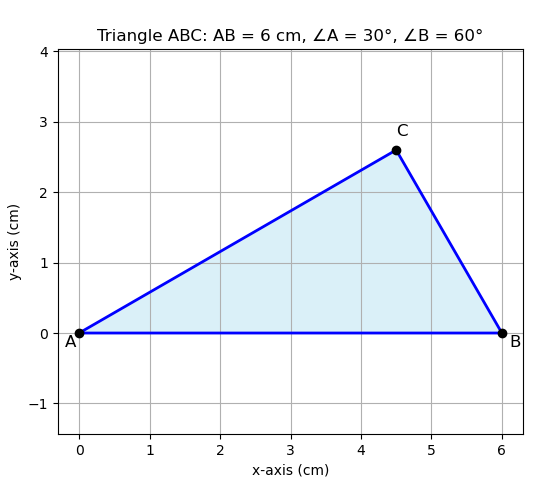
\includegraphics[width=0.6\linewidth]{figs/fig1.png}
        \end{document}
